\documentclass{standalone}
\usepackage{tikz}
\usepackage{subfigure}
\usetikzlibrary{backgrounds,automata}

\begin{document}
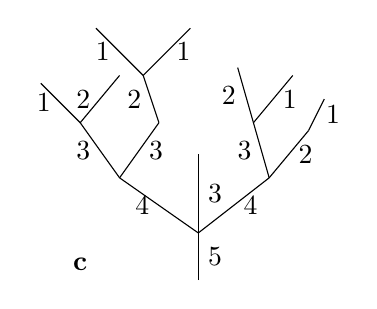
\begin{tikzpicture}
    \draw (-2, 2.5) -- (-1.5, 2);
    \path (-2, 2.5) -- (-1.5, 2) node[midway, left] {1};

    \draw (-1, 2.6) -- (-1.5, 2);
    \path (-1, 2.6) -- (-1.5, 2) node[midway, left] {2};

    \draw (-1.5, 2) -- (-1, 1.3);
    \path (-1.5, 2) -- (-1, 1.3) node[midway, left] {3};

    \draw (-1.3, 3.2) -- (-0.7, 2.6);
    \path (-1.3, 3.2) -- (-0.7, 2.6) node[midway, left] {1};

    \draw (-0.1, 3.2) -- (-0.7, 2.6);
    \path (-0.1, 3.2) -- (-0.7, 2.6) node[midway, right] {1};

    \draw (-0.7, 2.6) -- (-0.5, 2);
    \path (-0.7, 2.6) -- (-0.5, 2) node[midway, left] {2};

    \draw (-0.5, 2) -- (-1, 1.3);
    \path (-0.5, 2) -- (-1, 1.3) node[midway, right] {3};

    \draw (-1, 1.3) -- (0, 0.6);
    \path (-1, 1.3) -- (0, 0.6) node[midway, left] {4};

    \draw (0.5, 2.7) -- (0.7, 2);
    \path (0.5, 2.7) -- (0.7, 2) node[midway, left] {2};

    \draw (1.2, 2.6) -- (0.7, 2);
    \path (1.2, 2.6) -- (0.7, 2) node[midway, right] {1};

    \draw (0.7, 2) -- (0.9, 1.3);
    \path (0.7, 2) -- (0.9, 1.3) node[midway, left] {3};

    \draw (1.6, 2.3) -- (1.4, 1.9);
    \path (1.6, 2.3) -- (1.4, 1.9) node[midway, right] {1};

    \draw (1.4, 1.9) -- (0.9, 1.3);
    \path (1.4, 1.9) -- (0.9, 1.3) node[midway, right] {2};

    \draw (0.9, 1.3) -- (0, 0.6);
    \path (0.9, 1.3) -- (0, 0.6) node[midway, right] {4};

    \draw (0, 1.6) -- (0, 0.6);
    \path (0, 1.6) -- (0, 0.6) node[midway, right] {3};

    \draw (0, 0) -- (0, 0.6);
    \path (0, 0) -- (0, 0.6) node[midway, right] {5};

    \path (0, 0) -- (-1.5, 0) node[left, above] {\textbf{c}};
\end{tikzpicture}
\end{document}
